\chapter{Domain Model}
\label{chap:domain-model}

\npar The domain model is shown in figures \ref{fig:domain-left} and
\ref{fig:domain-right}. All concepts in the diagram can be looked up in the glossary (see
\ref{chap:glossary}, page \pageref{chap:glossary}).

\begin{figure}[H]
	\begin{centering}
		%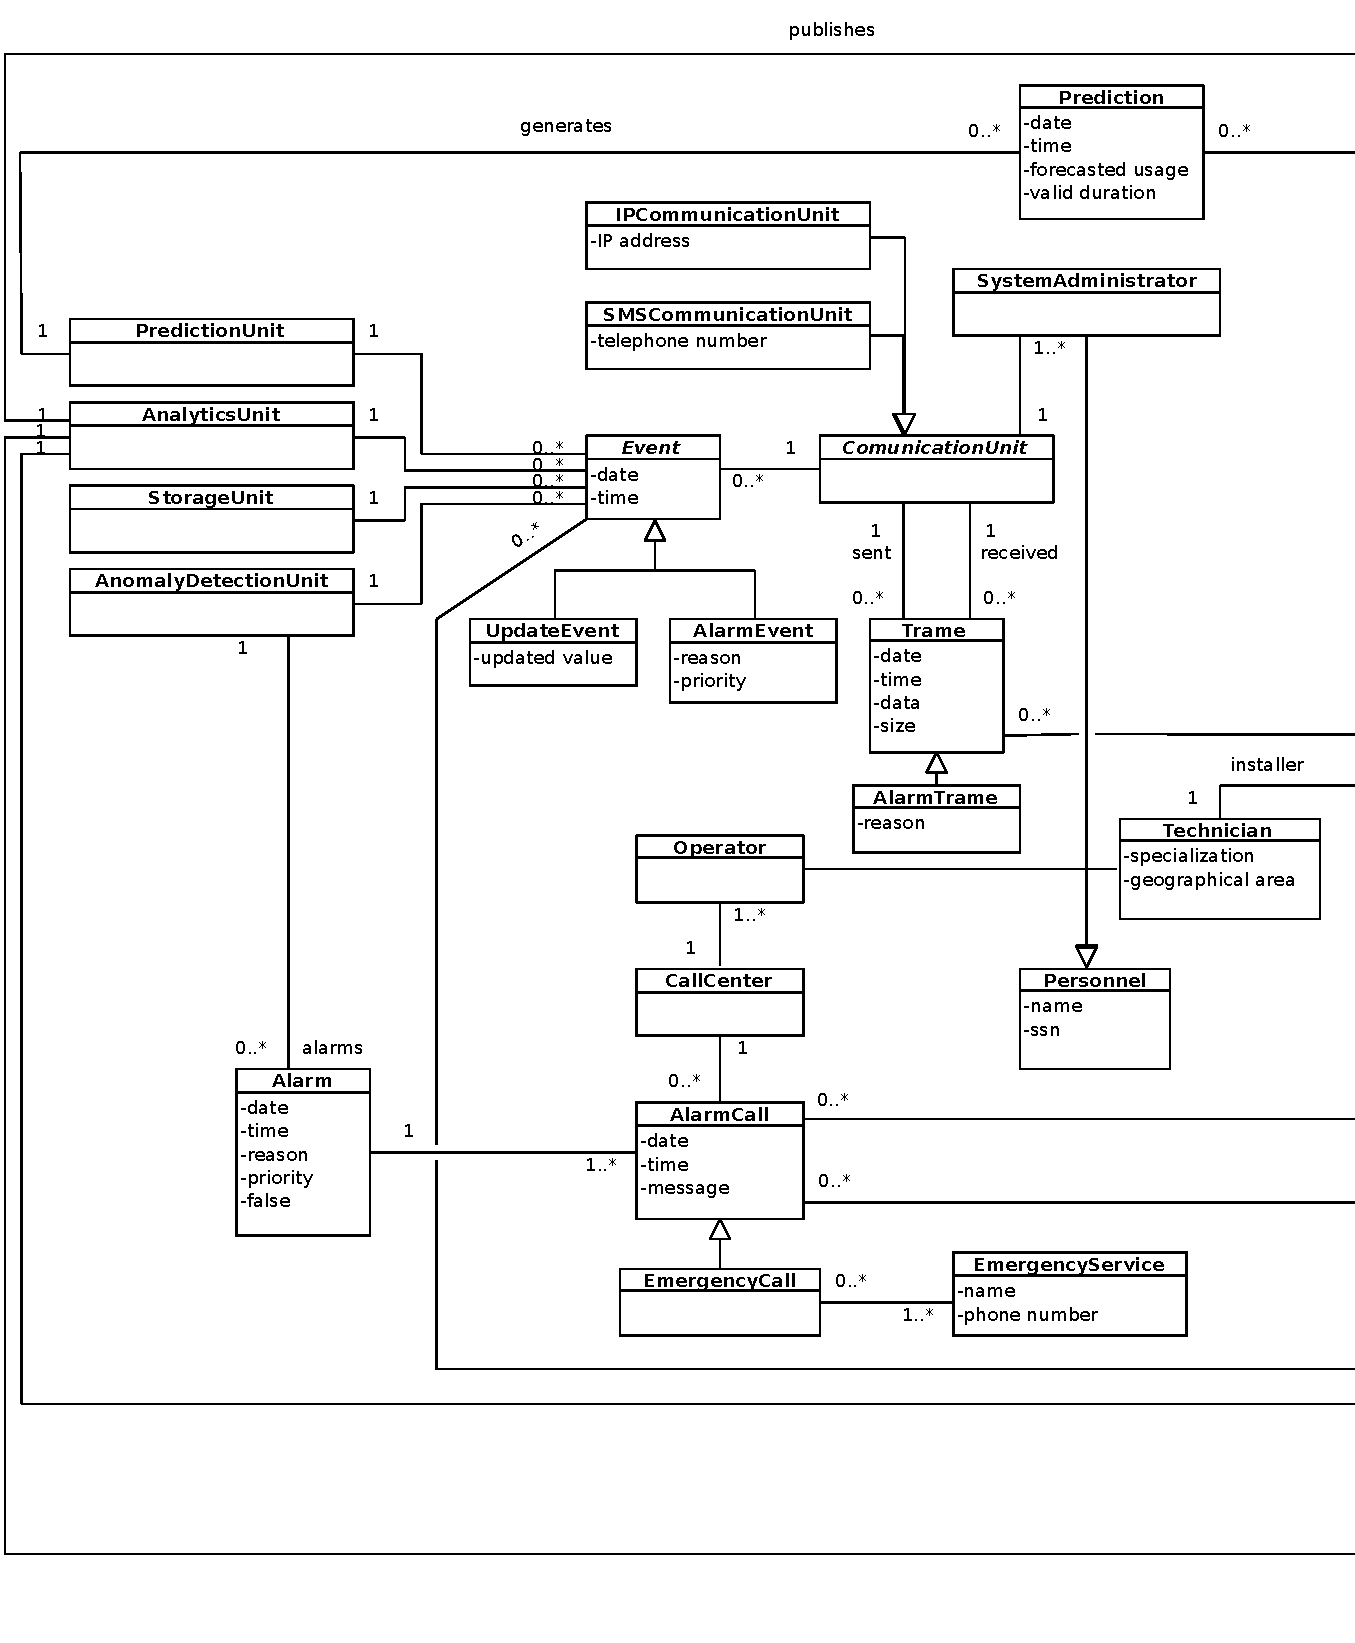
\includegraphics[width=\textwidth]{figs/domain-model-left.pdf}
		\caption{The left hand side of the full domain model}
		\label{fig:domain-left}
	\end{centering}
\end{figure}

\begin{figure}[H]
	\begin{centering}
		%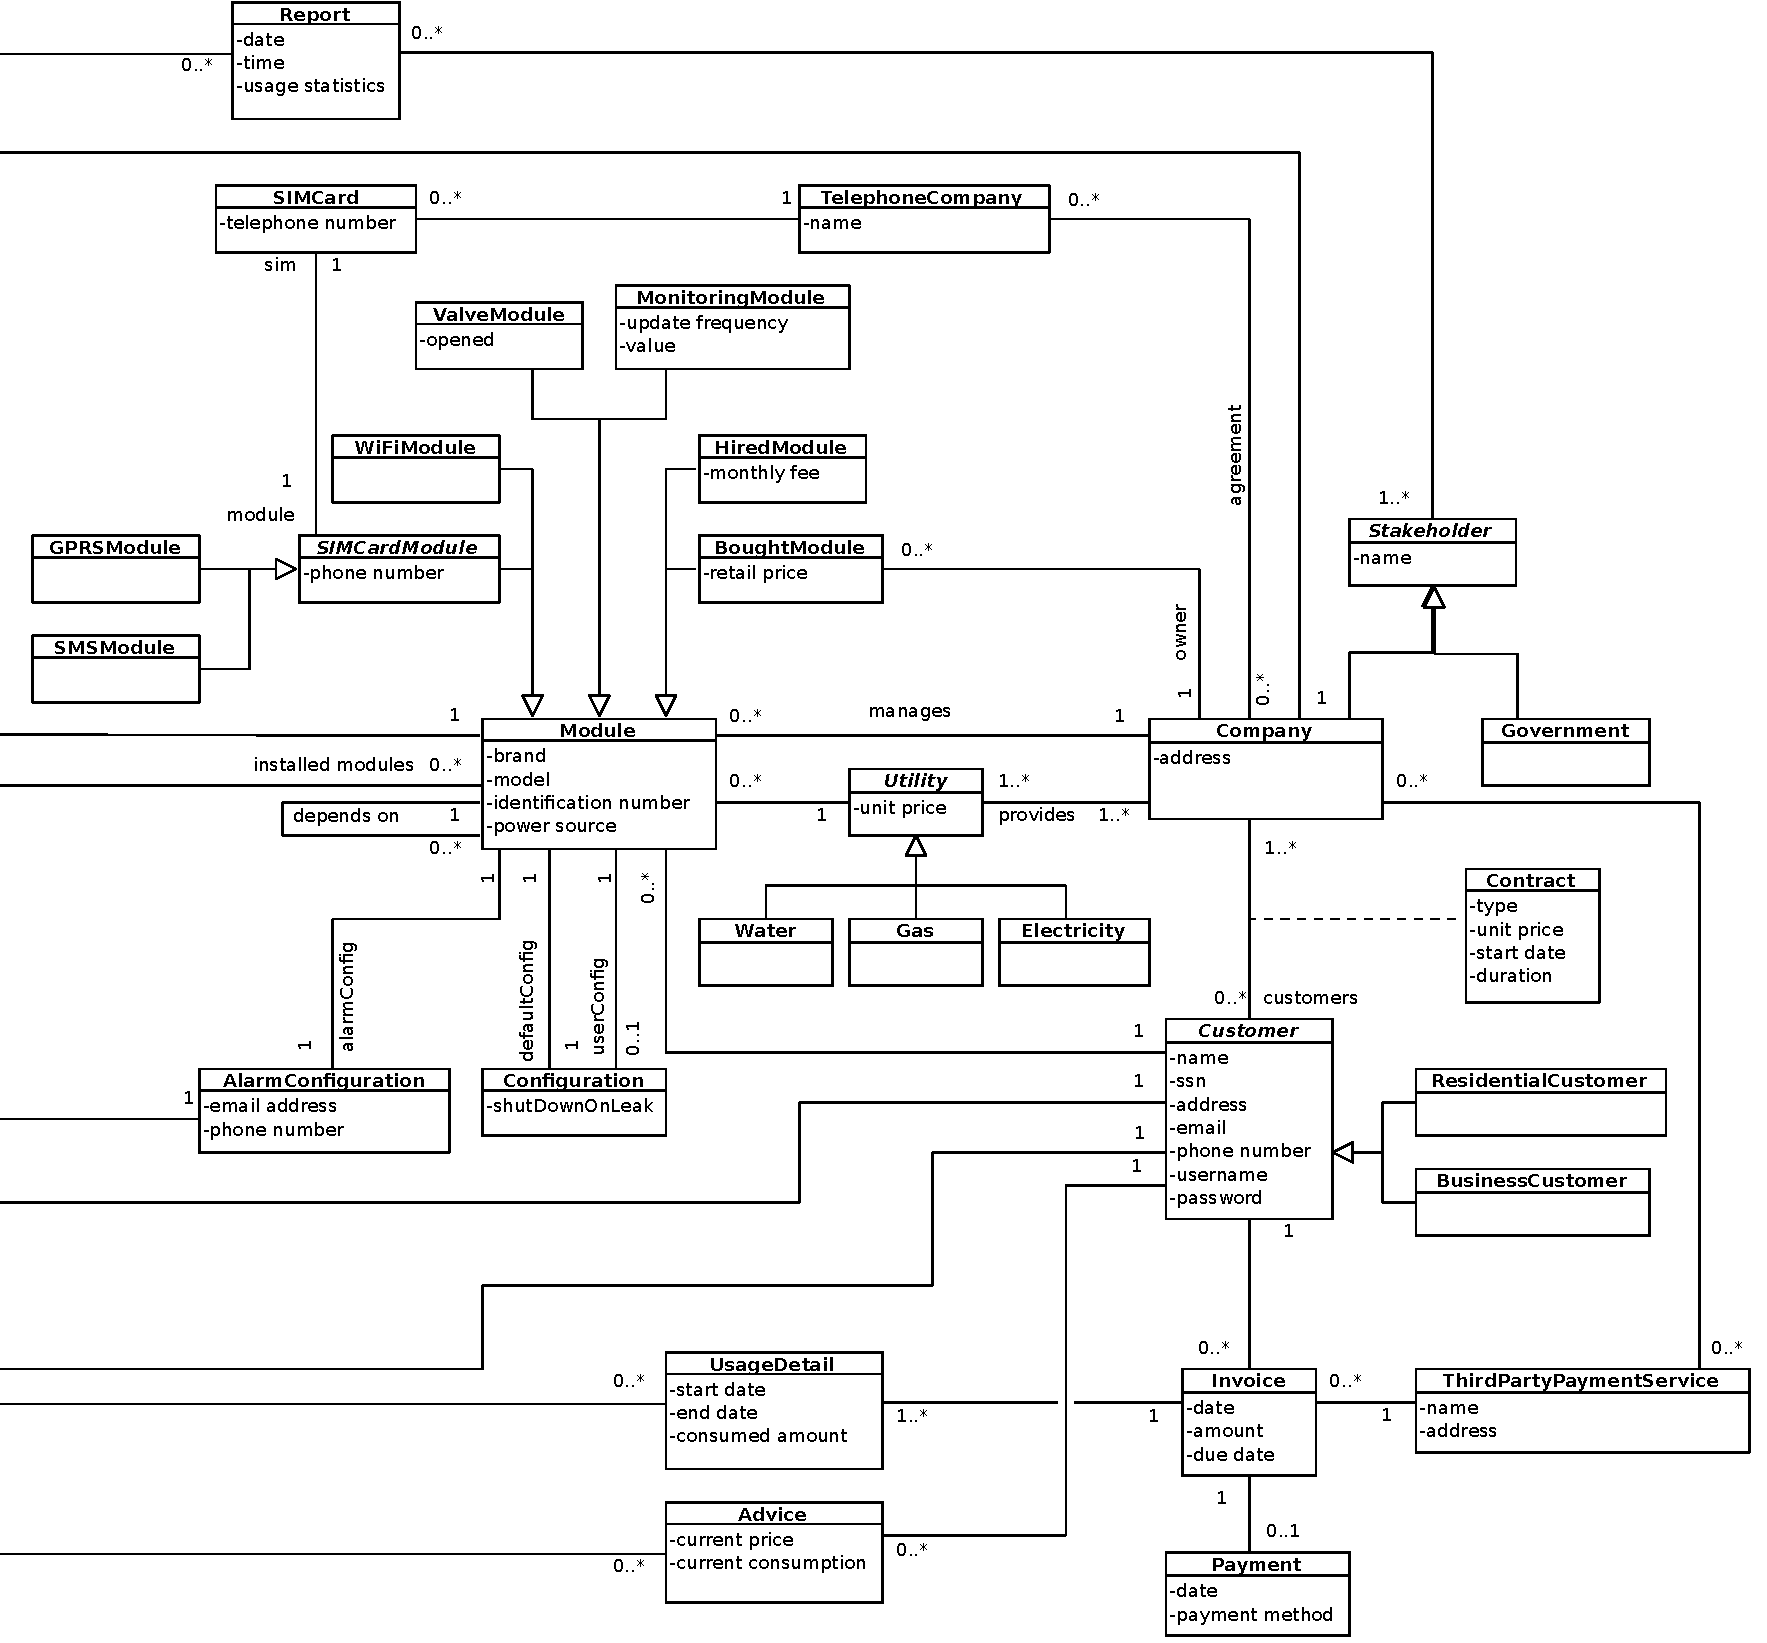
\includegraphics[width=\textwidth]{figs/domain-model-right.pdf}
		\caption{The right hand side of the full domain model}
		\label{fig:domain-right}
	\end{centering}
\end{figure}